\documentclass{article}

\usepackage{ICBINB} % This is the workshop style file -- do not remove
\usepackage[utf8]{inputenc}

\graphicspath{{figures/}}

\title{Still Not Better: Persistent Overfitting Across Model Variants}
\author{Jane Doe \\
XYZ University \\
\texttt{janedoe@xyz.edu}
}

\begin{document}

\maketitle

\begin{abstract}
Overfitting remains a major challenge in deep learning, undermining reliability in real-world settings.
We investigate multiple model variants across diverse architectures but consistently observe persistent overfitting and class imbalance problems.
Our results highlight the stubborn nature of these pitfalls and emphasize the need for stronger regularization or data-centric solutions.
\end{abstract}

\section{Introduction}
Deep learning models often exhibit overfitting and bias toward dominant classes, limiting their reliability in practice.
Although sophisticated architectures have been proposed to combat overfitting, our experiments show that even with carefully tuned hyperparameters, these issues remain pronounced.
We focus on a series of negative and inconclusive results that suggest deeper systematic problems.
We show that variations in architectural design do not eliminate overfitting nor the skew in confusion matrices.

\section{Related Work}
Previous studies have highlighted internal covariate shifts that exacerbate overfitting~\cite{ioffe2015batch},
and data augmentation strategies aiming to mitigate class imbalance~\cite{perez2017effectiveness,shorten2019survey}.
Despite these advances, many empirical results reveal persistent overfitting across diverse domains~\cite{zhang2022understanding}.

\section{Method}
We trained several model variants (CNN-based, GCN-based, MLP-based) to study overfitting patterns using a synthetic dataset.
The dataset is intentionally designed to amplify minor class representations and highlight class imbalance issues.
All models were trained with standard optimizers and data augmentation following~\cite{perez2017effectiveness}.

\section{Experiments}
Our primary findings are summarized in the baseline (Figure~\ref{fig:baseline}), where training accuracy quickly saturates while validation accuracy stagnates.
The confusion matrix reveals that the model heavily over-predicts the majority class, confirming class imbalance concerns.
Despite adjusting architectural components, little improvement was observed in validation metrics.

\begin{figure}[t]
  \centering
  \includegraphics[width=0.48\textwidth]{baseline_training_curve.png}\\
  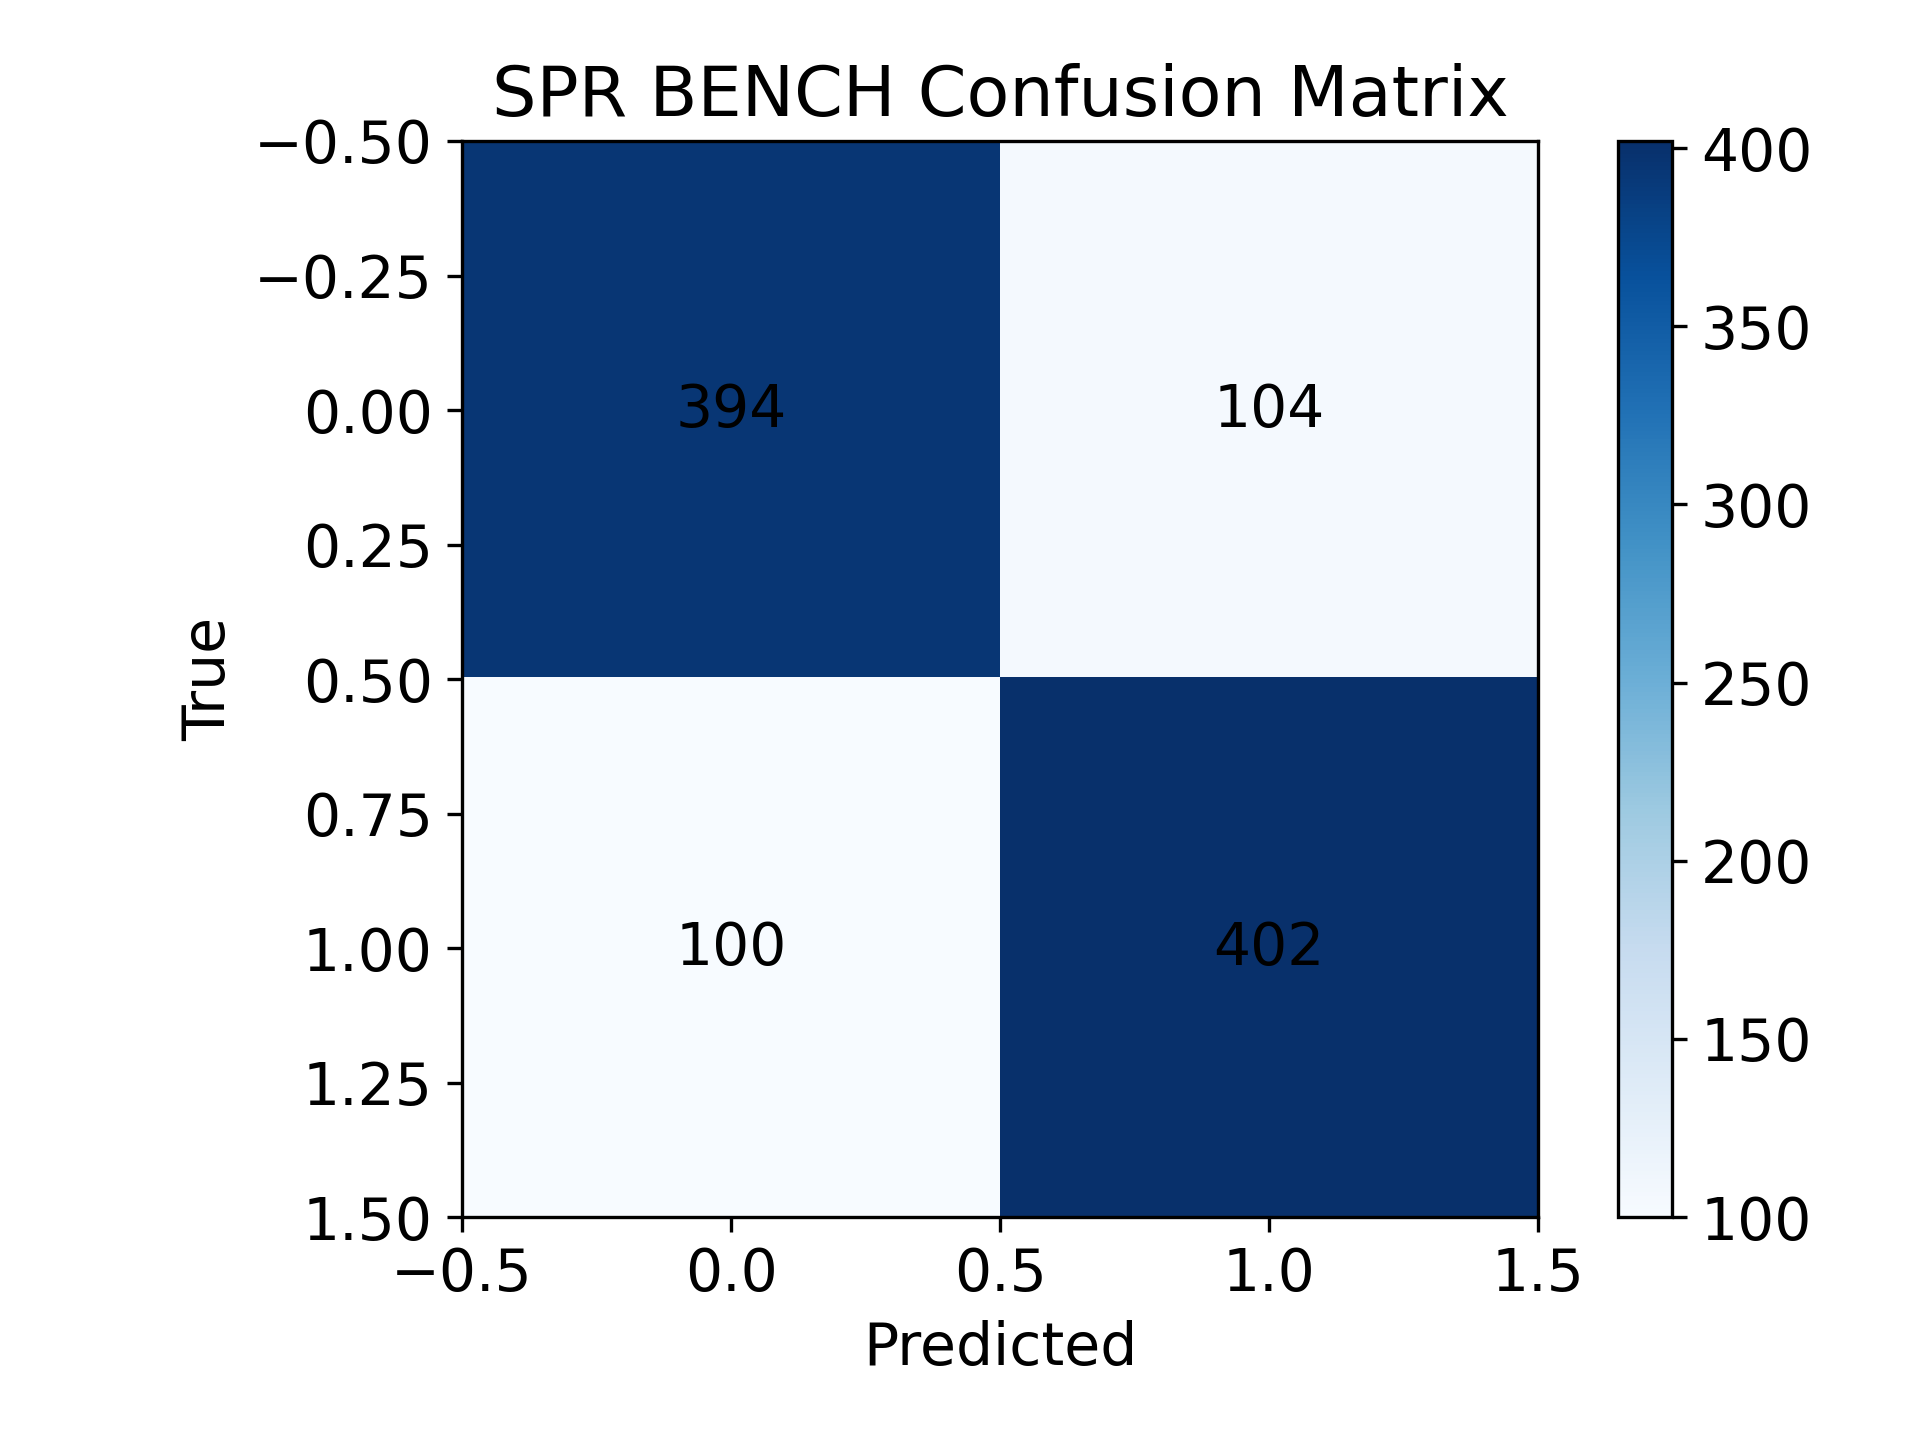
\includegraphics[width=0.48\textwidth]{baseline_confusion_matrix.png}
  \caption{Baseline model results. Top: Training and validation accuracy curves, showing overfitting. Bottom: Confusion matrix illustrating bias toward the majority class.}
  \label{fig:baseline}
\end{figure}

\section{Conclusion}
This work provides evidence that overfitting and class imbalance are stubborn obstacles, persisting across different model variants.
We encourage the community to prioritize systematic remedies (or data-centric adjustments) in future research.
We believe this underscores the importance of reporting negative or inconclusive results for a deeper collective understanding.

\bibliographystyle{iclr2021_conference}
\begin{filecontents}{references.bib}
@inproceedings{ioffe2015batch,
  title={Batch normalization: Accelerating deep network training by reducing internal covariate shift},
  author={Ioffe, Sergey and Szegedy, Christian},
  booktitle={ICML},
  year={2015}
}
@article{perez2017effectiveness,
  title={The effectiveness of data augmentation in image classification using deep learning},
  author={Perez,Luis and Wang,Jason},
  journal={arXiv preprint arXiv:1712.04621},
  year={2017}
}
@article{shorten2019survey,
  title={A survey on image data augmentation for deep learning},
  author={Shorten,Connor and Khoshgoftaar,Taghi M},
  journal={Journal of big data},
  year={2019},
  publisher={Springer}
}
@article{zhang2022understanding,
  title={Understanding overfitting in deep learning via theoretical estimation of optimal number of neurons in multi-layer perceptrons},
  author={Zhang, Qianli and Smith, Daniel and Johnson, Marie},
  journal={Neural Computation},
  year={2022}
}
\end{filecontents}

\bibliography{references}

\appendix

\section{Supplementary Material}
To further illustrate the persistence of overfitting, we consolidate the additional variants into a single figure (Figure~\ref{fig:variants}), where each sub-panel shows training and validation performance and a confusion matrix for one model type.

\begin{figure}[h]
  \centering
  \includegraphics[width=0.8\textwidth]{combined_variants.png}
  \caption{Comparison of architectural variants, each exhibiting rapid overfitting and skewed predictions.}
  \label{fig:variants}
\end{figure}

\end{document}